\documentclass[12pt,a4paper,twoside]{book}
\usepackage{graphicx}
\usepackage{setspace} %double spacing for text, single for captions, footnotes, etc.
%\usepackage{hypernat} %substitute for cite that allows hyperlinks
\usepackage{natbib} % substitute for 'hypernat' that works on Windows.
\usepackage[english]{babel}
\usepackage[utf8]{inputenc}
\usepackage{color}
\usepackage{hhline} % extended styles for tables
\usepackage{multirow}
\usepackage{subfigure}
\usepackage{acronym}
\usepackage{hyperref}
\usepackage{amsmath,amsmath,amssymb}
\usepackage{fancyhdr}
\usepackage{epsfig, amsmath}
\usepackage{algorithm}
\usepackage{algorithmic}
\usepackage{booktabs}


% general settings
\hypersetup{
linktocpage=true,
colorlinks=true,
linkcolor=blue,
citecolor=blue,
}
\definecolor{Hgray}{gray}{0.6}

\newenvironment{definition}[1][Definition]{\begin{trivlist}
\item[\hskip \labelsep {\bfseries #1}]}{\end{trivlist}}

\setlength{\topmargin}{0cm}
\setlength{\textheight}{23cm}
\setlength{\textwidth}{17cm}
\setlength{\oddsidemargin}{0cm}
\setlength{\evensidemargin}{0cm}
\setlength{\headheight}{1cm}

% indicates that 'sub-sub-sections' are numbered and appear in the index
\setcounter{secnumdepth}{3}
\setcounter{tocdepth}{2}

% settings for code
\renewcommand{\algorithmicrequire}{\textbf{Input:}}
\renewcommand{\algorithmicensure}{\textbf{Output:}}

%%%%%%%%%%%%
% DOCUMENT %
%%%%%%%%%%%%
\begin{document}

%\addbibresource{Dermatological-lesion-classification.bib} %Zotero bibliobrafy file

% cover page
\newpage
\thispagestyle{empty}

\baselineskip 2em

%\vspace*{1cm}

\centerline{
\includegraphics[width=0.6\textwidth]{images/UOC-logo}}
\begin{center}
\textsc{Open University of Catalonia (UOC) \
Master's Degree in Data Science \
}

%\centerline {\pic{UOC}{4cm}}

\vspace*{1.5cm}

\textsc{\Large MASTER'S THESIS}

\vspace*{0.5cm}

\textsc{\large Area: Medicine}

%\textbf{\Huge VirtualTechLab Model: }

\vspace*{2.0cm}

\textbf{\Large Dermatological lesion prediction}

\textbf{\large Classify dermoscopic among nine different diagnostic categories}

\vspace{2.5cm}
\baselineskip 1em

\baselineskip 2em
-----------------------------------------------------------------------------\

Author: Jesús González Leal\

Tutor: Jordi de la Torre Gallart\

Professor: Laia Subirats\

-----------------------------------------------------------------------------\

\vspace*{1.5cm}
Barcelona, \today

\end{center}

\newpage
\pagestyle{empty}
\hfill
\newpage
% abstract
\pagenumbering{roman}
\setcounter{page}{1}
\pagestyle{plain}

%%%%%%%%%%%%%%%%
%%% CREDITS %%%
%%%%%%%%%%%%%%%%
\chapter*{Credits/Copyright}

The dataset used in this work is protected by the CC-BY-NC licence \cite{cc_by_nc_license}.

\begin{figure}[ht]
\centering

\includegraphics[scale=1]{images/CC BY-NC license.png}
\end{figure}

\vspace{1cm}

This document, and its code, are licensed under Attribution-NonCommercial-NoDerivs 3.0 Spain (CC BY-NC-ND 3.0 ES) 

\href{https://creativecommons.org/licenses/by-nc-nd/3.0/es/}{3.0 Spain of CreativeCommons}.


\begin{figure}[ht]
\centering

\includegraphics[scale=1]{images/license.png}
\end{figure}




%%%%%%%%%%%%%
%%% RECORD %%%
%%%%%%%%%%%%%
\chapter*{FINAL PROJECT RECORD}

\begin{table}[ht]
\centering{}
\renewcommand{\arraystretch}{2}
\begin{tabular}{r | l}
\hline
Title of the project: & Dermatological lesion classification\\
\hline
Author's name: & Jesús González Leal\\
\hline
Collaborating teacher's name: & Jordi de la Torre Gallart\\
\hline
PRA's name: & Laura Subirats\\
\hline
Delivery date (mm/yyyy): & 02/2024\\
\hline
Degree or program: & Master’s degree in data science\\
\hline
Final Project area: & Medicine\\
\hline
Language of the project: & English\\
\hline
Code repository: & https://github.com/chus73/Dermatological-lesion-classification\\

\hline
Keywords & \textit Dermatological Diagnostic, Image classification, CNN  \\
\hline
\end{tabular}
\end{table}

%%%%%%%%%%%%%%%%%%%
%%% DEDICATION %%%
%%%%%%%%%%%%%%%%%%%
\chapter*{Dedication/Quote}

Dedicado a mis pequeños, la fuente de mi alegría. Espero serviros de inspiración y que podáis lograr todos vuestros sueños. 

%%%%%%%%%%%%%%%%%%%
%%% Acknowledgements %%%
%%%%%%%%%%%%%%%%%%%
\chapter*{Acknowledgements}

I would like to acknowledge the work of the International Sink Imaging Collaboration \cite{isic_web} in helping to reduce skin cancer mortality. 

I would also like to acknowledge the "Universitat Oberta de Catalunya" for giving me the opportunity to grow personally and professionally.

%%%%%%%%%%%%%%%%
%%% ABSTRACT %%%
%%%%%%%%%%%%%%%%
\chapter*{Abstract}
\addcontentsline{toc}{chapter}{Abstract}

\onehalfspacing

The skin is the largest organ in the body, as well as the first barrier for defending our inner organs against any aggression, besides helping the body to regulate its temperature. Considering the importance of the skin for human beings, it is necessary to examine skin lesions and because of that dermatologists use dermatoscopy, which is a device for illuminating and magnifying the area to be examined, to monitor any present injury.  

During recent past decades, enormous advances in AI medical field have experienced important improvements due to the use of deep networks. They are able to diagnose with reliability as well as speed. 

The following project presents the use of deep learning algorithms in order to classify nine different diagnoses such as melanoma, basal cell carcinoma, vascular lesion and others of this kind.



\vspace{1.5cm}

\textbf{Keywords}: dermatoscopy, carcinoma, skin lesion classification, CNN.

\newpage

\pagestyle{fancy}
\renewcommand{\chaptermark}[1]{ \markboth{#1}{}}
\renewcommand{\sectionmark}[1]{\markright{ \thesection.\ #1}}
\lhead[\fancyplain{}{\bfseries\thepage}]{\fancyplain{}{\bfseries\rightmark}}
\rhead[\fancyplain{}{\bfseries\leftmark}]{\fancyplain{}{\bfseries\thepage}}
\cfoot{}

% table of contents
\cleardoublepage
\phantomsection
\addcontentsline{toc}{chapter}{Table of Contents}
\tableofcontents
% list of figures
\cleardoublepage
\phantomsection
\addcontentsline{toc}{chapter}{List of Figures}
\listoffigures
% list of tables
\cleardoublepage
\phantomsection
\addcontentsline{toc}{chapter}{List of Tables}
\listoftables

\thispagestyle{empty}

\pagenumbering{arabic}

\pagestyle{fancy}
\renewcommand{\chaptermark}[1]{ \markboth{#1}{}}
\renewcommand{\sectionmark}[1]{\markright{ \thesection.\ #1}}
\lhead[\fancyplain{}{\bfseries\thepage}]{\fancyplain{}{\bfseries\rightmark}}
\rhead[\fancyplain{}{\bfseries\leftmark}]{\fancyplain{}{\bfseries\thepage}}
\cfoot{}

\onehalfspacing

% chapters of the document
\chapter{Introduction}
\label{chapter: introduction}

%%% SECTION

Skin diseases such as skin cancer,  affect a large number of people around the world. Many of them are associated with a social stigma because the lesions look impressive causing rejection towards people having them.  Others, such as melanoma, are also associated with a high mortality rate, which is gradually decreasing thanks to advances in its early detection. Premature diagnosis, especially when the disease is in its first stages, will help to improve its prognosis and evolution. As a contribution to improving skin disease detection, this work has used convolutional neural networks to classify eight different types of skin disease. 
The dataset used for this study is part of the 2019 International Skin Imaging Collaboration (ISIC). The previously mentioned association launches annual challenges to stimulate researchers in the detection and classification of skin diseases. In concrete, the data used in this paper relates to the eight specific skin diseases shown in figure \ref{fig: skin_lesions_sample}. The series of data have been obtained using dermoscopic techniques and they have been provided by different hospital contributions. The dermoscopic is widely used by dermatologists due that it improves the diagnosis of lesions compared with the naked eye.


\begin{figure}[ht]
    \begin{center}
        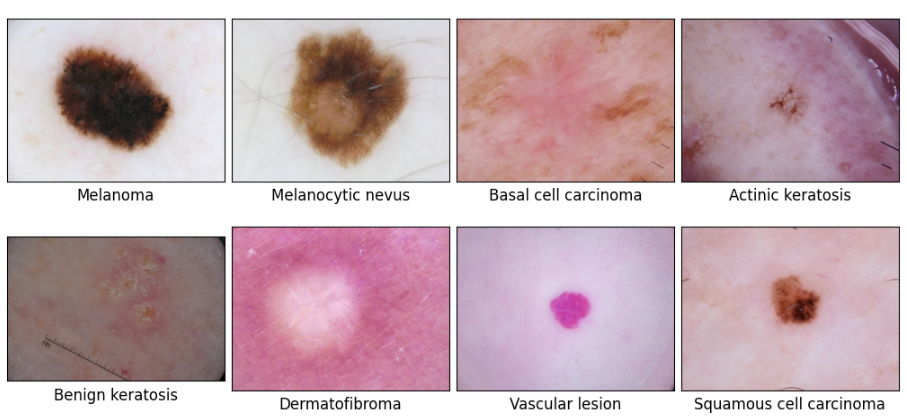
\includegraphics[scale=0.5]{images/Introduccion/skin_lesion_sample.png}
        \caption{Skin lesions sample}
    \label{fig: skin_lesions_sample}    
    \end{center}
\end{figure}


\section{Motivation}

%%%%%%%%%%%%%%%%%%%
%%% Motivation %%%
%%%%%%%%%%%%%%%%%%%
This journey towards the elaboration of this exciting work on dermoscopic classification of skin disease is a path that combines science, technology and medical care uniquely. 

Artificial Intelligence (AI) is bringing about a fourth industrial revolution that is already affecting our society. In concrete, its incorporation into medicine has a very significant impact on different medical areas (\cite{luciaclemares_que_2023} y \cite{apd_aplicaciones_IA_Medicina}) such as:

\begin{itemize}
    \item \textbf{A more accurate and organized diagnosis}: The use of advanced search techniques on large medical data sets allows for more accurate and reliable diagnostics. 
    \item \textbf{Faster and more efficient drug development}: Accelerating the research and development of new drugs.
    \item \textbf{Personalised care}: AI can customize treatment plans for each patient's individual needs optimizing, at the same time, effectiveness and minimizing side effects.
    \item \textbf{Images diagnostic more accurate and faster}. The worldwide name of AI will be recognized henceforth in this work as Deep networks. A part of these networks is specialized image recognition. They have a pattern detection capability that is by far superior to any human being. They can also make a diagnosis with very little delay. For the aforementioned reasons, it will be an essential tool for improving patient care and treatment. 
\end{itemize}

This last point is the core of the scope of this project. Personally, this project is much more than a task for ending a long master's journey. This job represents a challenge because working with large image files requires pre-processed data. In addition to this, the model to be developed is a classification one that should distinguish among nine different patterns.

It also represents an opportunity to imagine that my work could be helpful, one day, in the early detection of multiple skin diseases, and thus improve medical care and services.



\section{Goals}

%%%%%%%%%%%%%%%%%%%
%%% Goals %%%
%%%%%%%%%%%%%%%%%%%

This project's main objective is the classification of dermoscopic images in order to identify nine types of skin lesions. To achieve this a Convolutional Neural Network (CNN) will be created. This challenge can be separated into two goals.

\begin{itemize}
    \item On the one hand, to analyse the current \textbf{state of the art} in automatic medical detection by imaging.
    \item Secondly, to \textbf{classify these lesions into one of nine classes} to be studied.
\end{itemize}

In parallel, the dataset contains a metadata file. This information can help to segment the source information according to the types of dermoscopic techniques used. Therefore, this provides us with a \textbf{secondary objective} by allowing us to make a reliability ranking according to the technique used. 


\section{Methodology}

%%%%%%%%%%%%%%%%%%%
%%% Methodology %%%
%%%%%%%%%%%%%%%%%%%

For the implementation of this project, we will use the Cross Industry Standard Process for Data Mining or \textbf{CRISP-DM} methodology. This methodology consists of six phases that are cyclically carried out and it allows feedback to previous phases in order to complement the deficiencies of other phases. The following diagram (figure 1.1) shows the six-phase cyclical circuit to be used in this methodology.

\begin{figure}[ht]
    \begin{center}
        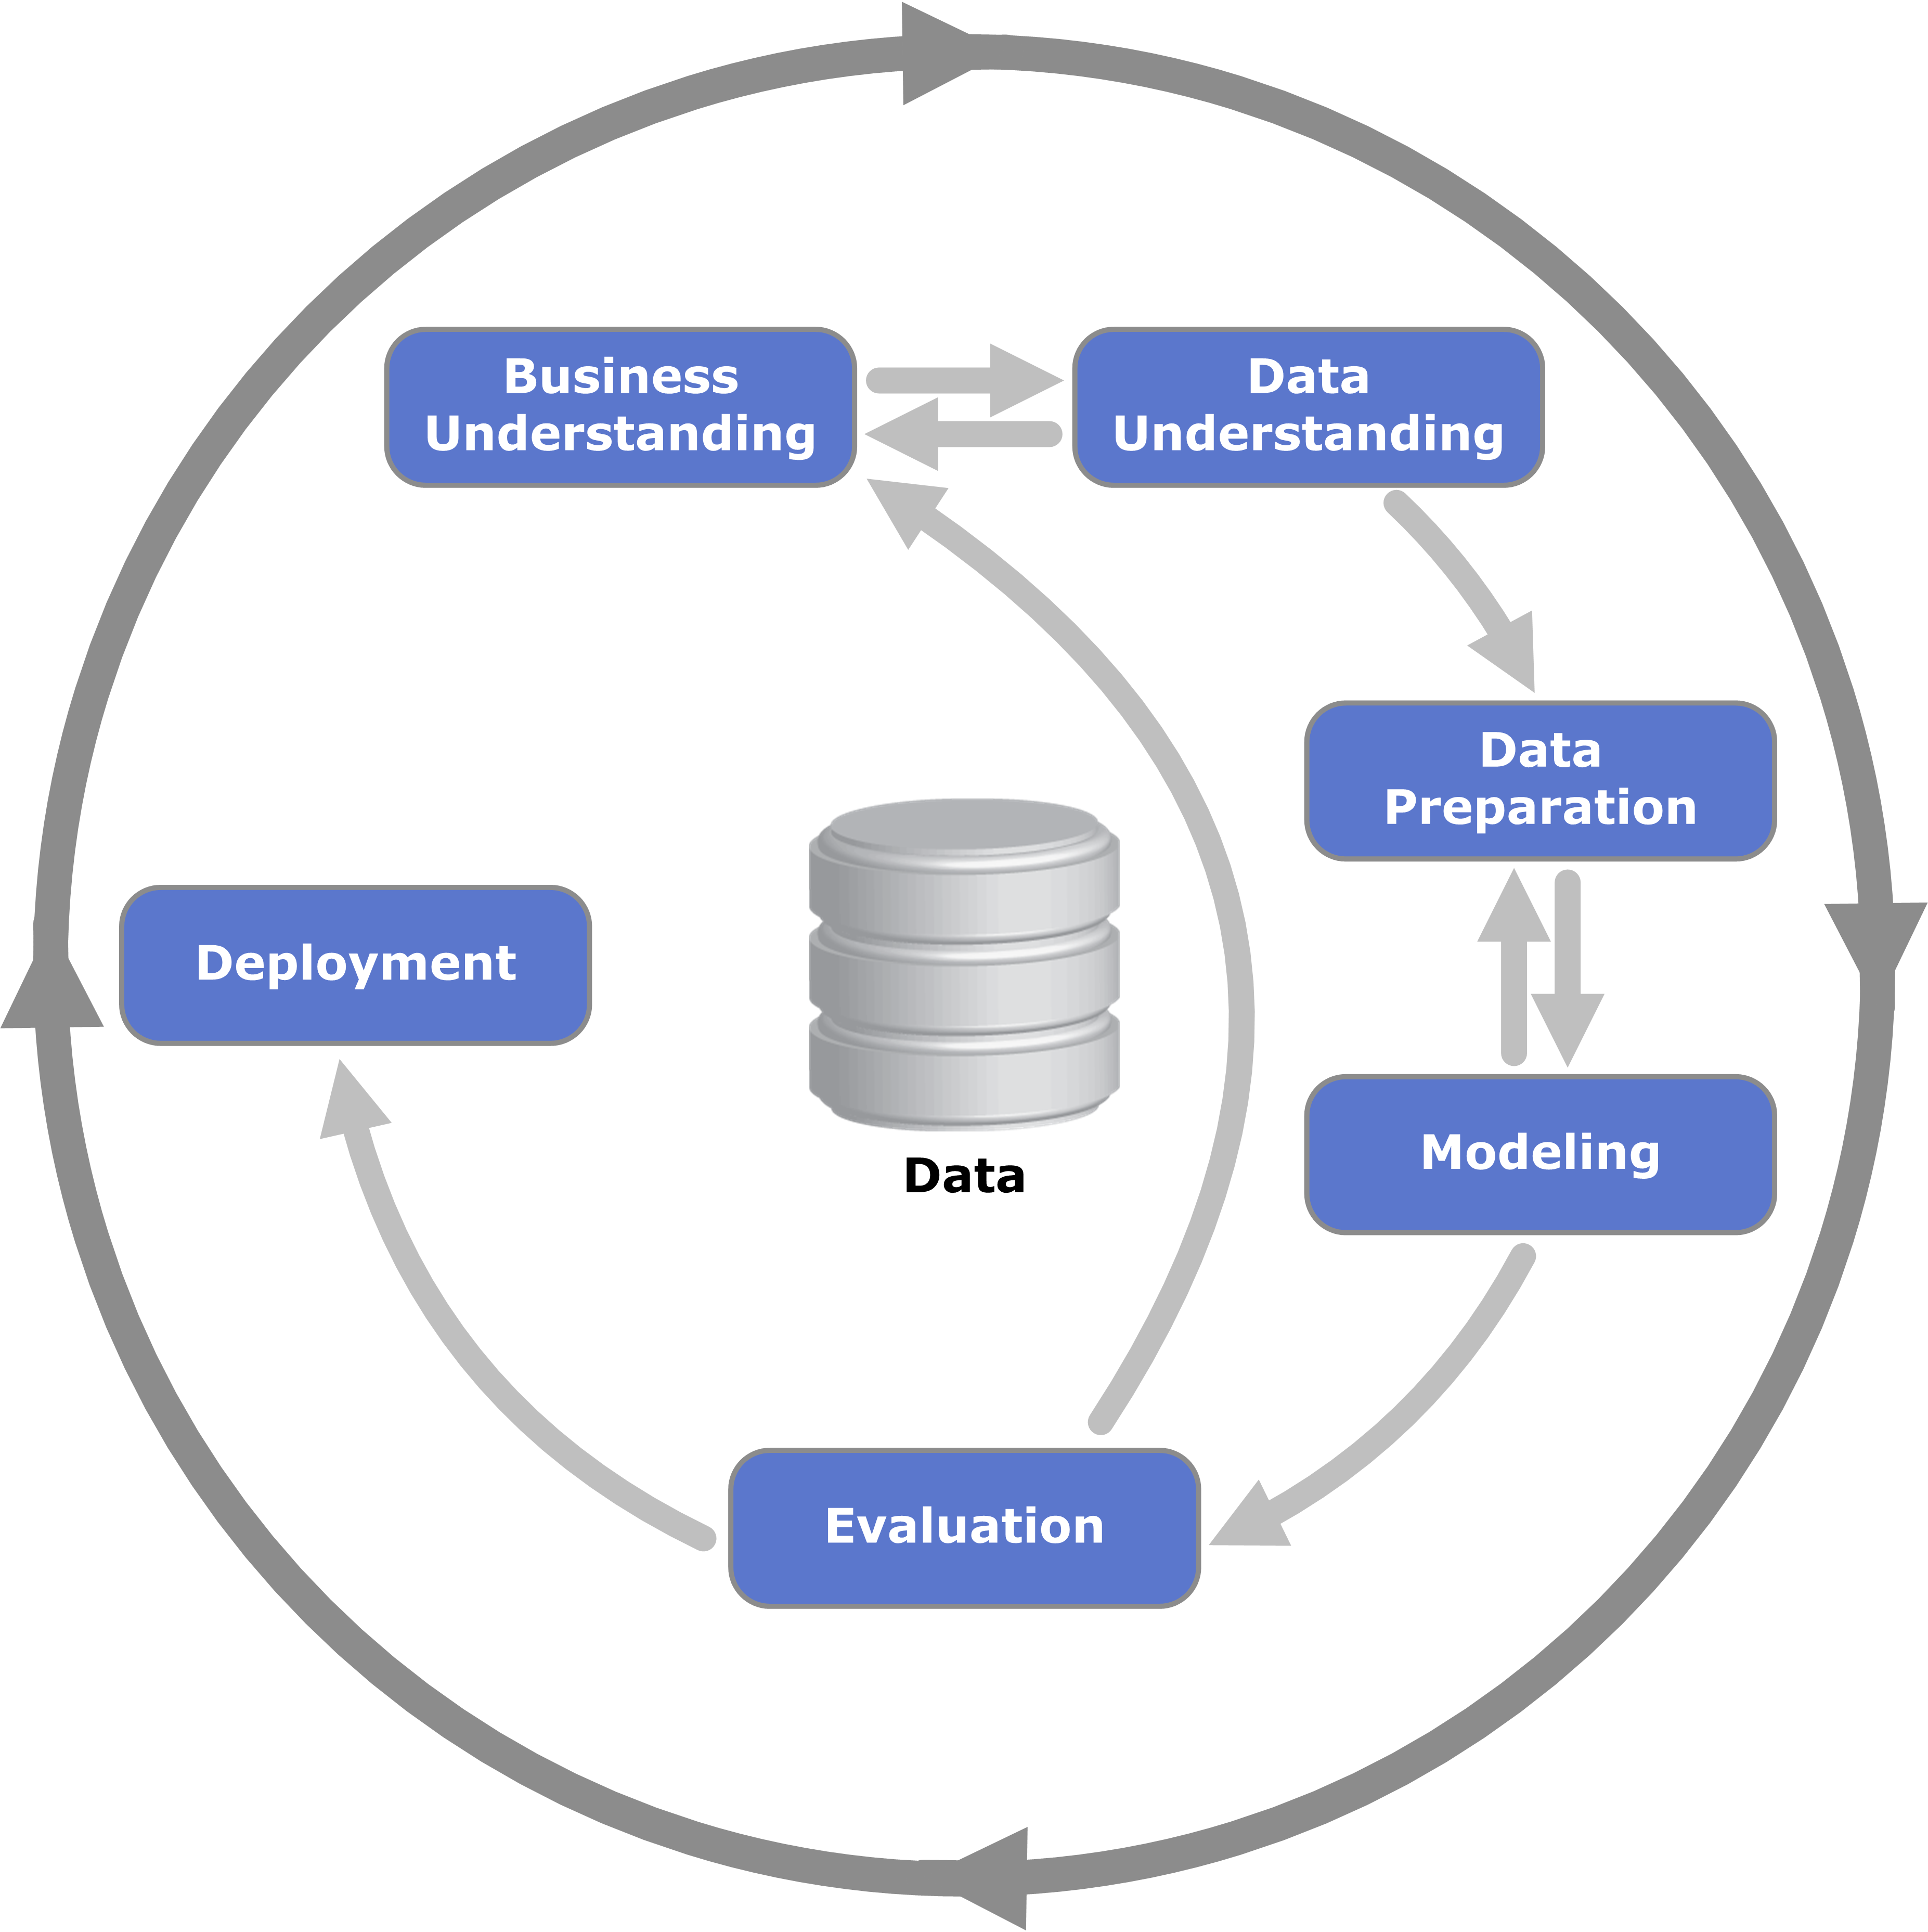
\includegraphics[scale=0.60]{images/CRISP-DM_Process_Diagram.png}
        \caption{Process diagram showing the phases of the CRISP-DM methodology}
    \label{fig:CRISP-DM}    
    \end{center}
\end{figure}


The methodology phases and the adaptation to the project are described below:

\begin{enumerate}
    \item \textbf{Business understanding}
    
    The first phase of the \textbf{CRISP-DM} model starts understanding the project's main objectives. These are mentioned in the \textbf{ Goals section} above. At this stage of the project, licensing costs are reviewed. Concerning licensing cost in this project there is \textbf{no associated licensing cost}, because the data is left under an open licence (see \textbf{Licensing section}). Furthermore, the project plan is also created during this phase (see \textbf{project plan section}).

    \item \textbf{Data understanding}
    
    Typically, this phase seeks to become familiar with the understanding of the data, identifying quality problems and discover hidden information or interesting subsets of the data to be processed. This allows to have point of view. A key aspect will be to verify the quality, in order to define all required strategies to address them. At the end of this phase, we will already have a conceptual data model.

    As the images to be used as a data source are produced in a medical environment, they are expected to be of high quality. However, this will be validated in the early stages of the project.

        
    \item \textbf{Data Preparation}

    In this section, applying the \textbf{CRISP-DM} method, a selection and integration of the main data together with their required attributes will be carried out. Moreover, data will be cleaned and formatted if required, looking for the main fields or characteristics of the data.

    Our project has the challenge of working with \textbf{large data input} (around 21 GB). Therefore, one of the first tasks will be \textbf{resizing} the data to reduce the size and work with a more manageable dataset. On the contrary, we will look at using some \textbf{data augmentation} techniques to help us avoid overfitting. 
    
    \item \textbf{Modelling}

    In this phase, the modelling techniques required to achieve an optimal data model will be applied. As it is  shown in the phase diagram, it is a phase that usually builds on the data preparation phase, either to solve problems or to enrich the data. Additionally to model building, some model evaluation techniques will be required. As a result, a test plan document will be done.

    
    \item \textbf{Evaluation}

    Once the objectives set requiered, during the initial phases have been obtained, an evaluation must be carried out to ensure that them were reached. This is done using the test plan designed in the previous phase. If necessary, the process will be reviewed and, depending on the results, the next steps will be planned. A benchmark well be carried out amont various models created, and the outstanding model is selected. 

    
    \item \textbf{Deployment}

    At the time, the model has passed all the tests and has been approved, it is required to define a plan for its deployment. Thus, creating a final model is not the end of the project, but rather a milestone within it. A model put into production environment it is necesary to monitor and maintain constantly. Along with the previous, it is advisable to publish results that help to understand whether the objectives initially requested in phase 1 have been achieved. It is quite common that after the project has been put into production, new expectations are generated that make the model (project) generated be reconsidered. This is why \textbf{CRISP-DM} describes the life cycle for the data mining project in a circular framework, where the output feeds back into a new cycle that seeks the continuous improvement of the business.

    Our project is part of a work that will develop a minimum viable product. Finally, the outstanding model will be run on the dataset test to obtain the final metrics.

After the project is structured by phases where no changes are expected in the definition of each one of them, and where the beginnings and ends of each phase are very well defined, a \textbf{waterfall model} is a better approach than other \textbf{agile strategies} for the project follow-up.

    
\end{enumerate}


\section{Planning}

%%%%%%%%%%%%%%%%%%%
%%% Planning %%%
%%%%%%%%%%%%%%%%%%%
The project has been structured in \textbf{five phases} or modules, which in turn are broken down into smaller tasks. This section describes the project's planning and its main milestones. 
\begin{itemize}
    \item \textbf{Module 1 - Project definition} 
    
    This module starts defining the project's plan: the relevant objectives of the project, the initial planning that will form the basis of the project, and the personal motivation to carry out the project on the chosen topic. During this phase, the form "Ethical and personal data protection protocol" will be filled out and presented.
    \item \textbf{Module 2 - State of Art}
    
    During this module time, we will carry out a research phase in which we will search for previous or current scientific work related to this project the main topic. 
    \item \textbf{Module 3 - Design \& implementation}
    
    The objectives of this activity are to implement the tasks necessary for the project's design and development according to the chosen scientific methodology. During this period, the progress made on it will be documented in order to complement the project document. 
    \item \textbf{Module 4 - Document redaction}
    
    This action's purpose is to prepare all the materials required for the presentation and final TFM (Master's Thesis) assessment. These materials include:
    
    \begin{enumerate}
        \item The Master's Thesis document
        \item An audiovisual presentation
    \end{enumerate}

    \item \textbf{Module 5 - Project defence}
    
    Finally, the last step of the Master's Thesis is to defend it before a board of examiners.
\end{itemize}

The following table shows each of the phases, namely: the start and end dates, as well as the estimated effort.


\begin{table}[H]
    \resizebox{\textwidth}{!}{%
    \begin{tabular}{@{}clcccc@{}}
        \toprule
        \textbf{Module}            & \textbf{Description}     & \textbf{Start Date}     & \textbf{End Date}     & \textbf{days} 
   & \textbf{Effort (h)} \\ \midrule
        \textbf{} 1 & Project definition & 09/27/23 & 10/10/23 & 13 & 26 \\
        \textbf{} 2 & State of Art & 10/11/23 & 10/24/23 & 13 & 26 \\
        \textbf{} 3 & Design \& Implementation & 10/25/23 & 12/19/23 & 55  & 110 \\
        \textbf{} 4 & Document redaction & 12/20/23 & 01/16/24 & 27  & 54 \\
        \textbf{} 5 & Project defence & 01/17/24 & 02/03/24 &  17 & 34 \\
        \bottomrule
    \end{tabular}%
    }
    \caption{Project Timetable.}
    \label{table:Timetable}
\end{table}



The time evolution of the project is shown by the following Gantt graph.

\begin{figure}[H]
    \begin{center}
        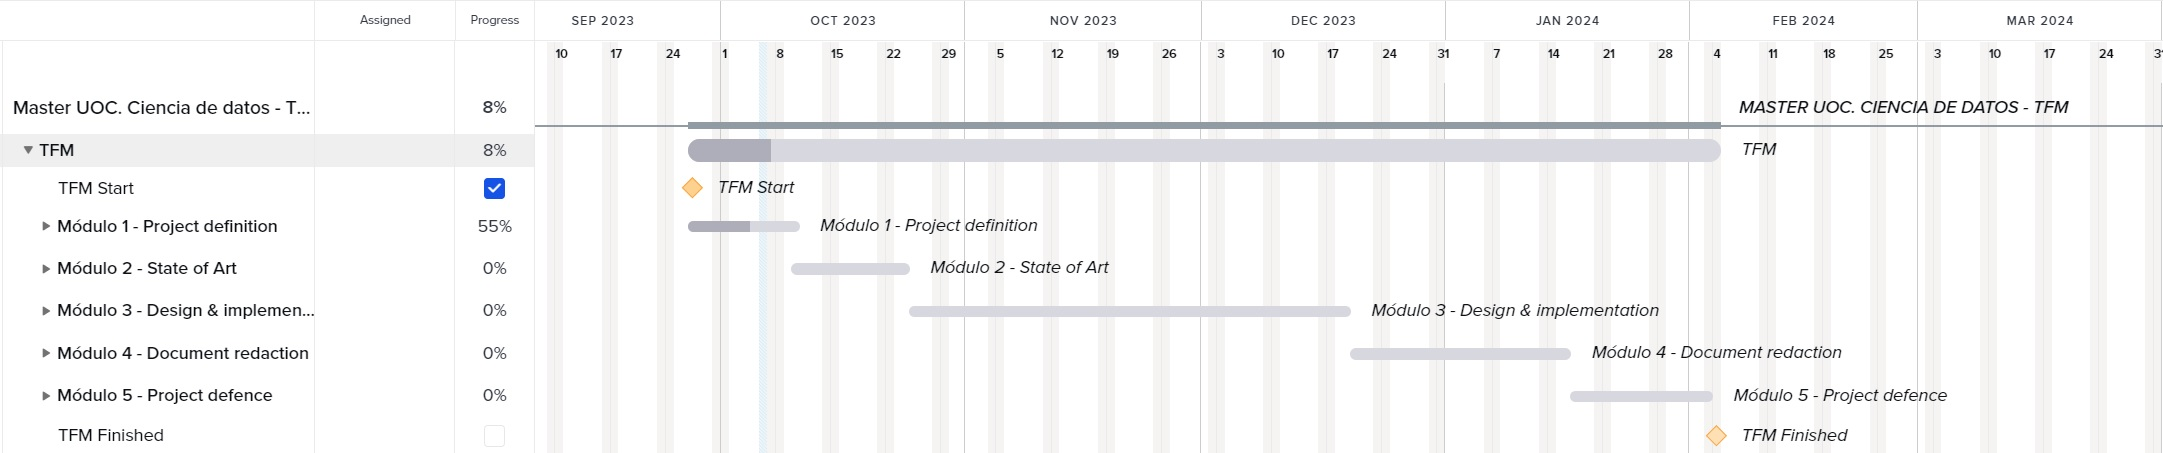
\includegraphics[scale=0.43]{images/TFM_Planing.jpg}
        \caption{Master's final project Gantt's chart}
    \label{fig:Gantt}    
    \end{center}
\end{figure}

\chapter{State of the Art}
\label{chapter: State of the Art}

%%% SECTION
Research into expert systems for image processing in medicine to support diagnosis has been in progress since the last decade of the last century \cite{beuscart_expert_1997}, \cite{chan_expert_1996}. Even though at the end of the 20th century we can already find diagnostic work based on neural networks \cite{wells_medical_1998}, the trend in research is to exploit the use of Machine Learning (ML) algorithms in image classification \cite{dreiseitl_comparison_2001}, \cite{dreiseitl_classifying_2000}. Thus, in the first half of the 21st century, research efforts are focused on improving the performance of ML algorithms by adding a \textbf{previous layer of feature selection} \cite{lee_machine_2009}. An example can be found in this text \cite{garnavi_computer-aided_2012}, the authors performed a benchmark with machine learning classifiers, measuring the impact of using a preprocess to extract texture, contour delineation and geometric properties of the melanoma lesion before moving to the classification stage.  The text concludes that the use of the three features makes the classifier perform better, with texture being the dominant feature to improve the accuracy metric. Feature extraction to allow discrimination and classification of samples is the main problem ML algorithms face when processing medical images, including dermoscopic images. In this area of medicine, the asymmetry, border, colours and dermoscopic rule (also known as \textbf{ABCD rule} in dermatology) or the Colour, Architecture, symmetry and homogeneity (\textbf{CASH rule}) is common to aid classification \cite{lee_machine_2009}. About this point, in 2012 \cite{6263297} we can find research where a complete feature extractor is built that makes use of a preprocessing stage for the delimitation of the lesion boundary, the symmetry on two axes, the geometry and the texture, feeding its output to four ML classifiers (Support Vector Machine (SVM), random forest, logistic model tree and hidden naive Bayes) with good results. In 2014, the use of a k-means algorithm for the separation of samples into colours, together with a logistic regression already achieved a sensitivity of 62\% and a specificity of 76\% \cite{6803866} and in 2015 \cite{abuzaghleh_noninvasive_2015}, the use of cascade SVM together with a filter for hair detection, a Gaussian low-pass filtering on each of the channels allows for higher accuracy, approaching 98 \%.

Although, as we have seen above, research in image processing using neural networks dates back to the end of the 20th century, it is from the first decade of the 21st century that developments based on this technology begin to emerge strongly. This is due to the use of graphics processing units (GPUs) to compute the calculations, to which tensor processing units (TPUs) were subsequently added, together with the provision of large labelled data sets and the commitment to innovation by large technology companies and institutions. Thus, in 2011, the famous paper "\textit{Building High-level Features Using Large Scale Unsupervised Learning}" \cite{le_building_2012} by Google engineers established a turning point in image processing by using neural networks for large-scale unsupervised learning on 31,000 images. Unlike the ML models seen above, neural networks belong to the group of unsupervised classifiers, where the system identifies the main features, without relying on manual supervision \cite{Le2011BuildingHF}.In contrast to the previous trend in ML, which added complexity to models by focusing on the feature extraction layer, with neural networks, the\textbf{ network itself learns to extract the most relevant patterns from the image}.

Within the set of types of neural networks, we find that there is a group with direct applications in image processing. We refer to \textbf{convolutional neural networks} (CNN) \cite{shiri_comprehensive_nodate} \cite{chen_review_2021}, which extract increasingly complex patterns as we go deeper into the layers of the network, increasing the level of abstraction of the object concerning the image. The network thus learns features and patterns that allow it to distinguish the object through training, accurately detecting those same patterns in other images not used during training. Each layer of the CNN neural network acts as a filter that detects a certain pattern in the image. Thus, it is easy to think that increasing the number of layers will increase the model's reliability. The price to pay is also an increase in the number of parameters to train and therefore, an increase in the training time of these models. This philosophy gives birth to the concept of \textbf{Deep Learning }(DL) \cite{noauthor_what_nodate} as a subfield within the area of ML.

\begin{figure}[ht]
    \begin{center}
        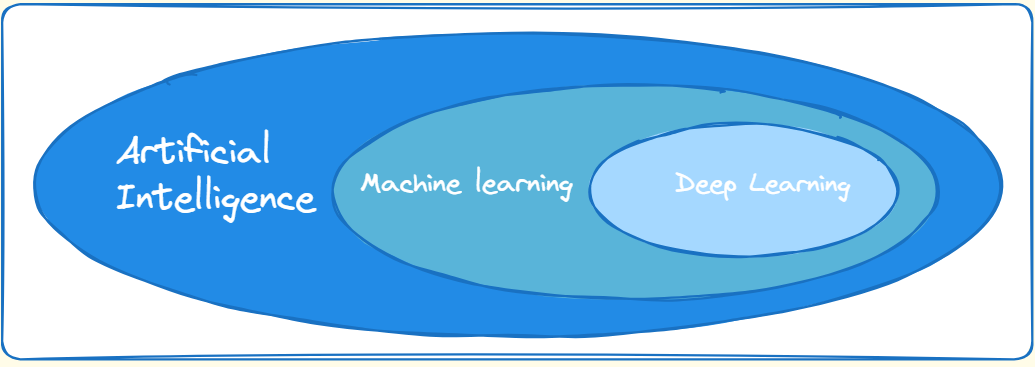
\includegraphics[scale=0.60]{images/AI_Group.png}
        \caption{Relationship between the subgroups that make up artificial intelligence.}
    \label{fig:IA Subgroup}    
    \end{center}
\end{figure}


The contemporary trend is the use of\textbf{intense networks} for image classification in the medical field, specifically in dermatology. However, incorporating more and more layers, in addition to increasing the number of parameters, has the disadvantage of degradation \cite{roy_effects_2023}. In this text \cite{7792699}, very deep neural networks of more than 50 layers have been used, with an initial segmentation process of the images before moving on to the classification stage. To overcome this problem of degradation in this type of network, they have used residual learning, with a Fully Convolutional 
Residual Network (FCRN). This type of network uses \textbf{residual learning}, \cite{laina_deeper_2016} the idea of which is to allow the layers of a neural network to learn the differences or residuals between the input and output. This is achieved by introducing hops in one or more layers of the network, which allows convergence in deep networks avoiding exploding or vanishing gradients \cite{wong_what_2021}.

Another current trend, in order to increase the accuracy of the models without increasing the number of layers too much,  is to revert to using a pre-processing layer to extract the main features before the classification. Thus in this work \cite{thamizhamuthu_deep_2023}, the pre-processing stage is based on the k-means machine learning algorithm, whose purpose is to segment the pixels by colour. In this sense, the aim of this layer is to isolate the lesioned region from the rest of the skin, and then go on to a feature extraction stage to determine the colour, the intensity of the information of each channel and the pattern of the lesion using different algorithms. The result is then passed to a feature selection stage that uses the statistical t-test to decide the importance of the features. These are classified by class to determine the image's dominant feature set, and the classified features feed a deep neural network. The results obtained are significant, reaching 99 \% Accuracy with 98.33 \% sensitivity. 

Another trend used in the last decade for the specific case of skin photo processing is the incorporation of a filter prior to the convolutional network to remove noise caused by hair in dermoscopic images.\cite{talavera-martinez_hair_2021}, \cite{bardou_hair_2022}, \cite{kaur_hairlines_2022}.

One of the problems facing the training of neural networks is the need for a very large set of quality data for training. In order to minimise the impact of having too little data, the \textbf{transfer learning} technique has been implemented in neural network architectures over the last decade \cite{rodrigues_new_2020}, \cite{wall_deep_2020}, \cite{abbes_deep_2021}, \cite{georgakopoulos_detection_2017}. The concept behind this technique lies underneath this architecture. Instead of training a model from scratch for a new task, transfer learning uses a pre-trained model from a previous task as a starting point. This pre-trained model has already learned useful features and data patterns that can be applied to the new task, which speeds up the training process and can result in better performance. 

Another problem commonly faced by CNNs is the risk of overfitting caused by limited data sources. It is common in these cases to incorporate \textbf{data augmentation} techniques in order to introduce variability and increase the number of data \cite{shorten_survey_2019}. These techniques consist of applying transformation methods to the image: rotation, translation, flipping, zoom or noise injection. 



% bibliography
\addcontentsline{toc}{chapter}{Bibliography}
\bibliographystyle{plain}
%\bibliography{references}
\bibliography{referencias}
%\bibliography{Dermatological-lesion-classification}

\end{document}
